\JWlone{Technical Prerequisites}
\label{sec:technical-prerequisites}

In this chapter the hardware inspected in this work is presented in detail. The
hardware used to inspect (the measuring device) will be depicted in a
chapter of its own (\ref{sec:measuring-device}).

% #  PRODUCTS  #################################################################
\JWltwo{Products}
\label{sec:hw-products}

\begin{itemize}

\item CPU: \JWPcpu{} (\emph{Sandy Bridge}\cite{wiki:snb} microarchitecture)

\item Mainboard: \JWPboard{} (using an external video controller)

\end{itemize}


% #  SANDY BRIDGE CHARACTERISTICS  #############################################
\JWltwo{Sandy Bridge Characteristics}
\label{sec:sandy-bridge}

In this section, characteristics of the Sandy Bridge microarchitecture are
described in detail.

\begin{figure}
  \centering
    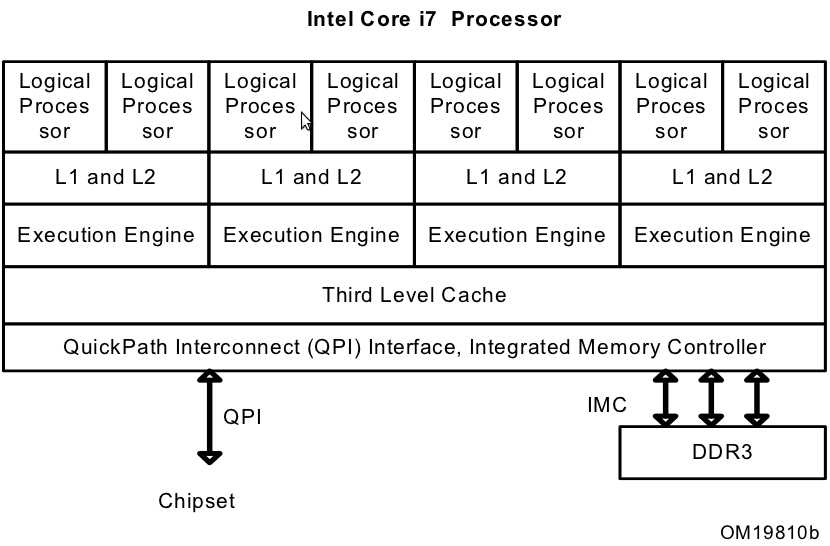
\includegraphics[width=\textwidth]{fig/intel-cache-orga.png}
  \caption{\JWPcpu{} cache organization (taken from \cite{intel2011softdev1})}
  \label{fig:cache-orga}
\end{figure}


%-  general  -----------------------------------------------------------------
\JWlthree{General}
\label{sec:sandy-brige-general}

The most evident characteristics of the \JWPcpu{} are the four cores (on one
chip) and the very uniform distribution of the caches (see figure
\ref{fig:cache-orga}). All caches except for the last-level cache (L3) are
present on each core \cite{fog11}. A short overview over the key features
follows (\cite{intel2011spec}):

\begin{itemize}

\item Number of cores: 4

\item CPU clock speed: \SI{3.4}{\giga\hertz}

\item L1 cache of \SI{64}{\kibi\byte} per core\cite{intel2011softdev1}

\item L2 cache of \SI{256}{\kibi\byte} per core\cite{intel2011softdev1}

\item shared L3 cache of \SI{8}{\mebi\byte}\cite{intel2011softdev1}

\end{itemize}


%-  PMU  -----------------------------------------------------------------------
\JWlthree{Performance Monitoring Unit}
\label{sec:pmu}

The CPU's \emph{Performance Monitoring Unit} (PMU) is present since the
Intel\TReg{} Pentium processor. Using this unit you are able to monitor several
of the CPU's performance parameters, originally meant for tuning system and
application performance (mostly used by compiler developers)
\cite{intel2011softdev3b}.

In prior work (\cite{bellosa2000benefits,snowdon2010operating,
weissel2002process,kellner03tempcontrol,bertran2010decomposable}) some of these
performance events have proven to be somehow related to the power consumption of
the CPU. As the selection of the events and the degree of their correlation to
energy highly varies between CPUs (or at least CPU microarchitectures) this has
been done again in this work. This time for the Intel\TReg{} Sandy Bridge
microarchitecture and in particular the \JWPcpu{}.

Examining the documentation \cite{intel2011events} approximalely 184 events have
been found available and usable. Because the CPU is only able to count eight
(four in Hyper-threading \cite{wiki:HT} mode) user-programmable performance
events at a time \cite{intel2011softdev1} the most useful events had to be
selected (see chapters \ref{sec:min-events} and \ref{sec:finding-useful-subset}
for a description of  the selection process). In addition to the eight (four)
events, the CPU provides three counters for fixed events, which will be counted
anyway: \JWctr{CPU\_CLK\_UNHALTED.REF\_TSC}, \JWctr{CPU\_CLK\_UNHALTED.THREAD}
and \JWctr{INST\_RETIRED.ANY}.

The selection, configuration and usage of these performance event counters is
done via special \emph{model specific registers} (MSRs), see
\cite{intel2011softdev3b} for the documentation. In this work a more high-level
approach via the \texttt{perf\_event}-API of newer Linux Kernels (some
documentation available at \cite{weaver2011perfevents}) and \JWtool{libpfm4}
(see chapter \ref{sec:standard-software}) has been used.


%-  architectural differences  -------------------------------------------------
\JWlthree{Architectural Differences between Sandy Bridge and Older Architectures}

The Intel\TReg{} \emph{Sandy Bridge} microarchitecture is a further development
of the Core and Nehalem architectures \cite{fog11}. Among other simplifications
of the branch prediction unit, the special loop predictor has been decontinued
presumably to reduce the overall pipeline length and to minimize the
misprediction penalties \cite{fog11}. For speed-improvements a micro-operation
($\mu$op) cache and macro-operation fusion have been introduced \cite{fog11}.
